\documentclass{article}
\usepackage[top=2cm, bottom=2cm, left=2cm, right=2cm]{geometry}
\usepackage[figurename=Figure]{caption}
\usepackage{graphicx} % Required for including pictures
\usepackage{float} % For tables and other floats
\usepackage{amsmath} % For math
\usepackage{amssymb} % For more math
\usepackage{fullpage} % Set margins and place page numbers at bottom center
\usepackage{paralist} % paragraph spacing
\usepackage{listings} % For source code
\usepackage{subfig}   % For subfigures
\usepackage{enumitem} % useful for itemization
\usepackage{circuitikz}
\usepackage{setspace} % to control the linespace
\usepackage{fancyhdr} % for the head and foot of pages
\usepackage{tikz} % draw pictures
\usepackage{wrapfig} % wrap figure
\usepackage{kantlipsum}
\usepackage{epstopdf}
\usepackage{color}
\definecolor{dkgreen}{rgb}{0,0.6,0}
\definecolor{gray}{rgb}{0.5,0.5,0.5}
\definecolor{mauve}{rgb}{0.58,0,0.82}
\lstset{frame=tb,
  language=Matlab,
  aboveskip=3mm,
  belowskip=3mm,
  showstringspaces=false,
  columns=flexible,
  basicstyle={\small\ttfamily},
  numbers=left,
  numberstyle=\tiny\color{gray},
  keywordstyle=\color{blue},
  commentstyle=\color{dkgreen},
  stringstyle=\color{mauve},
  breaklines=true,
  breakatwhitespace=true,
  escapeinside=``,
  tabsize=4,
  extendedchars=false 
}

% Set the head and foot of pages
\pagestyle{fancy}
\fancyhf{}
\rhead{120090272}
\chead{MAT3007 Assignment 2}
\lhead{Chuqiao Feng}
\rfoot{Page \thepage}

% The title of homework
\begin{document}
\rmfamily 
\hrule
\begin{center}
	\vspace{.4cm}
	{\textbf { \huge MAT3007 Assignment 2}}
\end{center}
\setlength{\baselineskip}{20pt}
\noindent
{\textbf{Name:} \ Chuqiao Feng \hspace{\fill} \textbf{Due Date:} February 25th 2022, 12:00 PM \\ 
{\textbf{Student Number:} \ 120090272 \hspace{\fill} \textbf{Assignment:} Assignment 2 \\
\hrule

% the question 1
\section*{Problem 1}
\subsection*{Solution:}
\large
1.\quad False \\ 
Reason: In some cases, LP can be feasible but optimal value is unbounded.\\
Example: \, minimize:  $c^Tx = [1, -1][x_1, x_2]^T$ \\
\hspace*{60pt}subject to: \, $Ax=b \Rightarrow [-1, 1, -1][x_1, x_2, x_3]^T = 0$\\
\hspace*{120pt} $x_1, x_2, x_3 \geq 0$ \\ 
In this case, the graph of LP is as below.\\
and in this case, the optimal value is feasible but unbounded, so the answer is False.\\ 
\begin{wrapfigure}{r}{5cm}
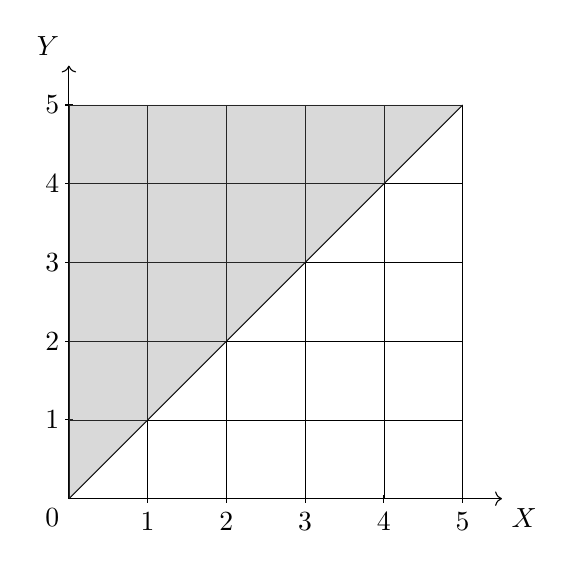
\begin{tikzpicture}
  \draw[help lines, black] (0,0) grid (5,5); % the web lines
  \draw [->] (0,0)--(5.5,0) node[below right] {$X$};
  \draw [->] (0,0)--(0,5.5) node[above left] {$Y$};
  \node[below left] at (0,0) {0};
  \foreach \i in {1,...,5}
  \draw (\i,-0.05)--++(90:0.1) node[below=1mm]{\i};
  \foreach \i in {1,...,5}
  \draw (0.05,\i)--++(180:0.1) node[left=-0.5mm]{\i};
  \draw[color=black ,domain=0:5]plot(\x,\x);
  \fill[thick,fill opacity=0.3][gray, domain=0:5, variable=\x]
    (0, 0)
    -- plot ({\x}, {\x})
    -- (0, 5)
    -- cycle;  
  \end{tikzpicture}
\end{wrapfigure}
2. \quad False \\ 
Reason: More than m variables can be positive.\\
Example: \, minimize: $c^Tx = [-1, -1][x_1, x_2]^T$ \\
\hspace*{60pt}subject to: $[1, 1, 1, 1][x_1, x_2, x_3, x_4]^T = 0$\\
\hspace*{120pt} $x_1, x_2, x_3, x_4 \geq 0$ \\ 
In the solutions of this linear program, $x_1+x_2=1$ and both larger than 0, in this case 2 variables are positive, which is larger than the scale of A for m=1, so the answer is False.\\
~\\ 
3. \quad True \\ 
Reason: If there is more than one optimal solution, then there are uncountably many optimal solutions.\\ 
Proof: \, minimize: $c^Tx$ \\
\hspace*{45pt}subject to: $Ax = b$\\
\hspace*{105pt} $x \geq 0$ \\ 
For feasible set is a convex set, objective function is linear.\\ 
Assume that $x_1, x_2$ are two optimal solutions of a multi-solution linear program with $x_1 \neq x_2$.\\ 
So we can have: $Ax_1 = Ax_2 = b$, and exist an $x_3$ in convex set such that $x_3=\lambda x_1+(1-\lambda)x_2$\\ 
multiply the equation with matrix A: $Ax_3=\lambda b +(1-\lambda)b=b \Rightarrow Ax_3 = b$\\ 
also $c^Tx_3= \lambda c^Tx_1 + (1-\lambda)c^Tx_2=c^Tx_1=c^Tx_2$\\
so we can infer from the equation that $x_3$ is also an optimal solution, and so as others.\\
So, if there is more than one optimal solution, then there are uncountably many optimal solutions, the answer is True.

~\\
\begin{wrapfigure}{r}{5cm}
  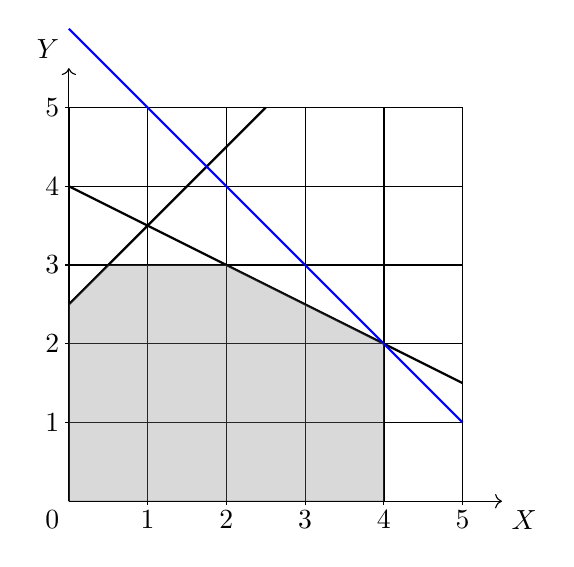
\begin{tikzpicture}
    \draw[help lines, black] (0,0) grid (5, 5); % the web lines
    \draw [->] (0,0)--(5.5,0) node[below right] {$X$};
    \draw [->] (0,0)--(0,5.5) node[above left] {$Y$};
    \node[below left] at (0,0) {0};
    \foreach \i in {1,...,5}
    \draw (\i,-0.05)--++(90:0.1) node[below=0.5mm]{\i};
    \foreach \i in {1,...,5}
    \draw (0.05,\i)--++(180:0.1) node[left=-0.5mm]{\i};
    \draw[color=black ,domain=0:2.5, thick]plot(\x,\x+2.5);
    \draw[color=black ,domain=0:5, thick]plot(\x,-\x/2 + 4);
    \draw[color=black ,domain=0:5, thick]plot(\x,3);
    \draw[-,black, thick] (4,0) -- (4,5);
    \draw[color=blue, domain=0:5,  thick]plot(\x, -\x+6);
    \draw[fill=gray,opacity=0.3] (0,2.5) -- (0.5,3) -- (2,3) -- (4,2) -- (4,0) -- (0,0)-- cycle;
\end{tikzpicture}
\end{wrapfigure}
% the question 2
\section*{Problem 2}
\subsection*{Solution:}
maximize: \quad $x_1+x_2$ \\ 
subject to: \, $-x_1+x_2 \leq 2.5$, \quad $x_1+2x_2 \leq 8$\\ \hspace*{70pt} $ 0 \leq x_1 \leq 4, $\quad $0\leq x_2 \leq 3$ \\ 
The graph of the LP is as below,\\ Active constraints: $x_1 \leq 4 $ and $x_1+2x_2 \leq 8$\\ 
Vertices of feasible region: (0,2.5),(0.5,3),(2,3),(4,2),(4,0),(0,0)

% the question 3
\section*{Problem 3}
\subsection*{Solution:}
1. \; the standard from: \\ \, minimize: \, $-x_1-4x_2-x_3$\\ 
subject to: \, $2x_1+2x_2+x_3+s_1$ \quad \quad \, =4\\
\hspace*{70pt}$x_1$\quad \quad \quad \, $-x_3$\quad \quad \quad$-s_2$=1\\ 
\hspace*{70pt}$x_1,x_2,x_3,s_1,s_2 \geq 0$\\ 
2. \; Write the constraints as: $Ax=b \Rightarrow $
$\begin{bmatrix}
2&2&1&1&0\\1&0&-1&0&-1
\end{bmatrix}$ $[x_1 x_2 x_3 s_1 s_2]^T$ = $\begin{bmatrix} 4\\1 \end{bmatrix}$\\
Solution = x = $A^{-1}_{B_(m)}b$\\
The indices: $[A_1,A_2],\;[A_1,A_3],\;[A_1,A_4],\;[A_1,A_5],\;[A_2,A_3],\;[A_2,A_5],\;[A_3,A_4],\;[A_3,A_5],\;[A_4,A_5]$\\
Basic Solutions: $[1,1,0,0,0],\;[\frac{5}{3},0,\frac{2}{3},0,0],\;[1,0,0,2,0],\;[2,0,0,0,1],\;[0,\frac{5}{2},-1,0,0],\;[0,2,0,0,-1],\;\\ $\hspace*{85pt}$[0,0,-1,5,0],\;[0,0,4,0,-5],\;[0,0,0,4,-1]$\\ 
Basic Feasible Solutions: $[1,1,0,0,0],\;[\frac{5}{3},0,\frac{2}{3},0,0],\;[1,0,0,2,0],\;[2,0,0,0,1]$\\ 
Values: $5,\,\frac{7}{3},\,1,\,2$\\ 
So the Basic Solutions and Basic Feasible Solutions are above.\\ 
3. \; From problem 2 we infer that the optimal solution is $x_1=x_2=1,x_3=0$, and the optmal value is 5.

\newpage ~\\ 
% the question 5
\section*{Problem 5}
\subsection*{Solution:}
The plot of the points are as below:\\
\begin{wrapfigure}{r}{11cm}
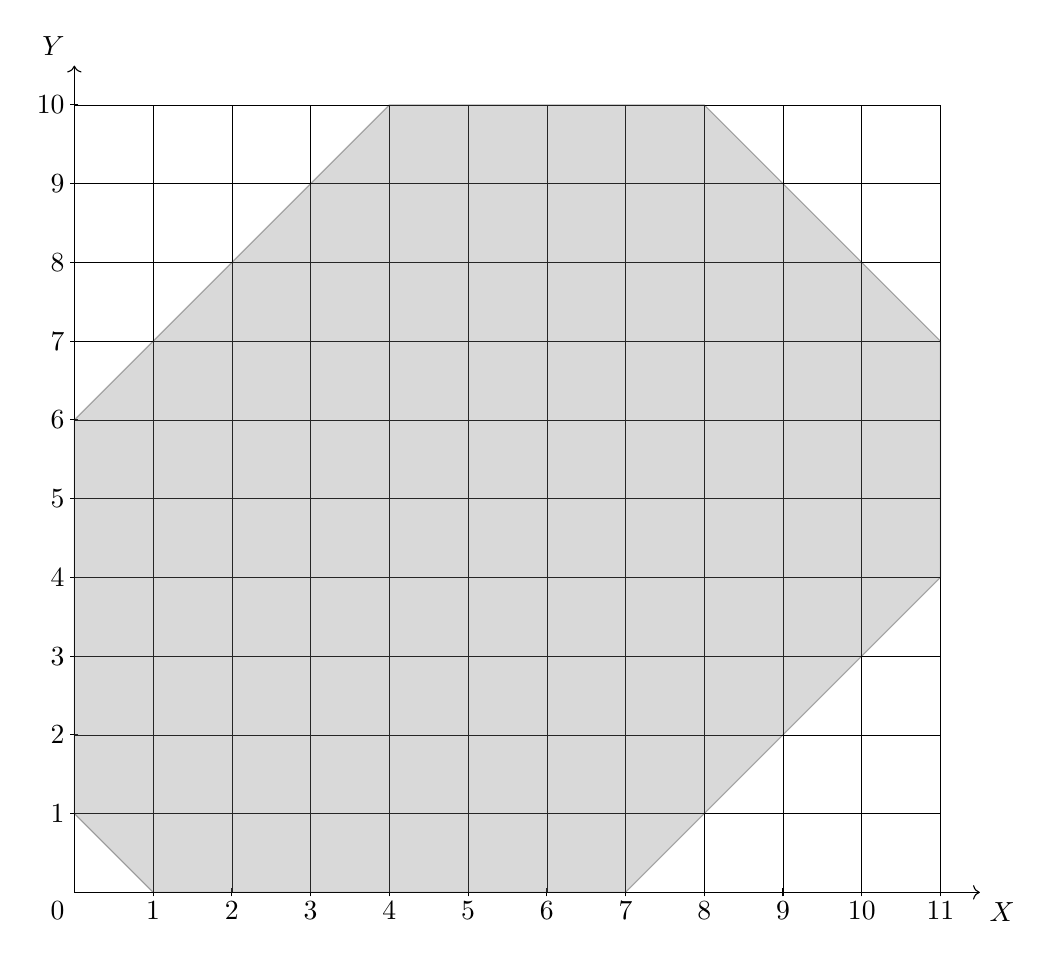
\begin{tikzpicture}[node distance=0.1cm]
    \draw[help lines, black] (0,0) grid (11, 10); % the web lines
    \draw [->] (0,0)--(11.5,0) node[below right] {$X$};
    \draw [->] (0,0)--(0,10.5) node[above left] {$Y$};
    \node[below left] at (0,0) {0};
    \foreach \i in {1,...,11}
    \draw (\i,-0.05)--++(90:0.1) node[below=0.5mm]{\i};
    \foreach \i in {1,...,10}
    \draw (0.05,\i)--++(180:0.1) node[left=-0.5mm]{\i};
    \draw[fill=gray, opacity=0.3] (0,1) -- (0,6) -- (4,10) -- (8,10) -- (11,7) -- (11,4)-- (7,0) -- (1,0)-- cycle;
  \end{tikzpicture}
\end{wrapfigure}
The functions of the constraints are:\\
$-x_1+x_2\leq 6$\\ $x_2\leq 10$\\$x_1+x_2\leq 18$\\$x_1\leq 11$\\$x_1-x_2 \leq 7$\\$x_2 \geq 0$\\$-x_1-x_2\leq -1$\\
~\\
So we can generate LP:\\
~\\
minimize: -r\\ 
subject to:\\
\quad A * y <= b;\\
\quad A * (repmat(y,1,8) + Direction' * r) <= repmat(b,1,8);\\
\quad r >= 0;\\ 
~\\
In the above equations, Direction is an matrix consists the information of direction.\\ 
And the constraints are:\\ 
b=[0,6,10,18,11,7,0,-1]\\
$A = \begin{bmatrix}
  -1&-1&0&1&1&1&0&-1\\0&1&1&1&0&-1&-1&-1
\end{bmatrix}^T$\\ 
solved by the software, the optimal center is at about(5.4, 4.8), and max radius r = 4.5962.\\ 
\newpage
~\\
% the question 4
\section*{Problem 4}
\subsection*{Solution:}
Solved by the sofware we find the optimal solution is: [0, 0, 5, 5, 5]
It means that if we purchase security 3, 4, 5, we will at least have 1 dollar profit



[The code of Q4 and Q5]:
\begin{lstlisting}
price = [0.75; 0.35; 0.40; 0.75; 0.65];
share_limit = [10; 5; 10; 10; 5];
payoff = [1, 1, 1, 0, 0;
          0, 0, 0, 1, 1;
          1, 0, 1, 0, 1;
          1, 1, 1, 1, 0;
          0, 1, 0, 1, 1];
results = eye(5);

cvx_begin quiet
variables x(5) outcome;
    minimize  -outcome;
    subject to:
        0<= x <= share_limit;
        w = x' * (payoff * results - repmat(price, 1, 5));
        repmat(outcome, 1, 5) <= w;
cvx_end
\end{lstlisting}
% \newpage~\\
\begin{lstlisting}
A = [-1,  0;
       -1,  1;
        0,  1;
        1,  1;
        1,  0;
        1, -1;
        0, -1;
       -1, -1];
b = [ 0;
       6;
      10;
      18;
      11;
       7;
       0;
      -1];
Direction = [1,          0;
             0,          1;
            -1,          0;
             0,         -1;
     sqrt(1/2),  sqrt(1/2);
     sqrt(1/2), -sqrt(1/2);
    -sqrt(1/2),  sqrt(1/2);
    -sqrt(1/2), -sqrt(1/2)];

cvx_begin quiet
variables r y(2); % generate variables r and y
    minimize -r;
    subject to:
        A * y <= b;
        A * (repmat(y,1,8) + Direction' * r) <= repmat(b,1,8);
        r >= 0;
cvx_end
\end{lstlisting}



\end{document}